\acresetall
\chapter{Introduction}\label{ch:intro}

Back in 1999, Joseph Mitola III coined the term \ac{CR}\cite{Mitola1999} as a way to enhance the \ac{SDR} capabilities by the means of a dynamic model that, based on human intervention, improved the flexibility of devices by making them fully configurable and capable of adapting to the communication system's needs, suitable to react to the changes in the environment. A formal definition for the \ac{CR} concept provided at \cite{Haykin2005} encloses the term nicely by describing it as a wireless system that is \emph{intelligent and aware of its surroundings}, whilst being able to learn, adapt and react to changes in the ambience, by modifying its operation parameters such as the transmission power, the modulation scheme, and its carrier frequency in real-time. Analogously, Jondral \cite{Jondral2005} adopts the short definition for \ac{CR} as "an \ac{SDR} that additionally senses its environment, tracks changes, and possibly reacts upon its findings", becoming an autonomous unit with the potential of using the spectrum efficiently.\\

\ac{CR} systems are intended to be immersed in a network, where it interacts with other systems that could be cognitive or non-cognitive radios. According to \cite{Goldsmith}, \ac{CR} is grouped under three paradigms: underlay, overlay and interweave. The \emph{Underlay Paradigm} allows the \ac{CR} system to operate under acceptable levels of interference, determined by an interference threshold. Here, the \ac{CR} is commonly called a \ac{SU}, providing priority to the other systems in the network which it should not significantly interfere, known also as \ac{PU}. In the \emph{Overlay Paradigm}, the cognitive transmitter knows information about the other transmitters in the network, such as their codebooks and modulation schemes. In addition, this model assumes that message that is being transmitted is known by the \ac{CR} when transmission by a non-cognitive system is initiated. This provides the cognitive system with multiple choices on how to use this information: for instance, it can be used to mitigate or completely cancel a possible interference happening in the network during transmission. Additionally, the cognitive system could also retransmit this message to other non-cognitive systems in the network, acting as a relay and, effectively, assist increasing the \ac{SNR} of the non-cognitive system to a level equivalent to the possible decrease due to the interference caused by \ac{CR} transmissions. The \emph{Interweave Paradigm}, or opportunistic communication, identifies temporary space-time-frequency gaps where it can intelligently allocate its transmission, increasing the available resource utilization and minimizing the interference with other active users. Hybrid schemes are also actively being developed \cite{Wu2007} \cite{Kaushik2015} \cite{Wunsch2017a}, where characteristics from different paradigms are combined in order to achieve an effective use of the available communication's resources.\\

The main characteristic required to apply any of the aforementioned paradigms is awareness, being it in regards to location, spectrum, time, etc. Awareness is achieved by the means of \emph{the cognition cycle} \cite{Mitola1999}, shown in Fig.~\ref{fig:cognition_cycle}, which enfolds the way the \ac{CR} parses the stimuli from the outside world in order to plan accordingly the proper reactions. This cognition cycle revolves around the following concepts:

\begin{figure}[htb]
    \centering
      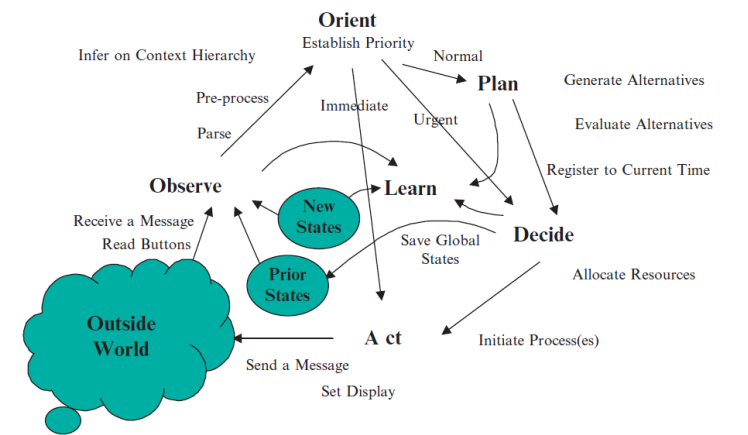
\includegraphics[width=0.8\textwidth]{figures/cognition_cycle.png}
      \caption{The cognition Cycle\cite{Mitola1999}}
      \label{fig:cognition_cycle}
\end{figure}

\begin{itemize}
    \item Observation: the \ac{CR} receives any signals from the external world, which can contain any type of information that the system can use in its favor and the favor of a better use of its resources.
    \item Orientation: The \ac{CR} determines the priority from the received signal as well as the type of reaction based on it.
    \item Planning: results from a normal-level priority, where a plan is generated and the sequence of actions to be taken are established.
    \item Decision: selects among the plan candidates the best proposal and allocates the necessary resources for its carrying-out.
    \item Acting: initiates action based on the previous taken decisions.
    \item Learning: is an integration of observations and decisions, based on past and current states that are compared with expectations. When an expectation is met, the system achieves effectiveness. When not, observations are recorded and kept for further learning.
\end{itemize}

These aspects of \ac{CR} come in handy when trying to solve one of the current major issues of communication systems: spectrum scarcity. The access to radio spectrum is highly regulated by government agencies such as the \ac{Ofcom}, the \ac{FCC} and the \ac{ITU}, and its access has been historically granted to the highest bidder on so-called \emph{spectrum auctions} \cite{Jondral2005} \cite{Staple2004}. Therefore, the seek of new technologies that allow a more efficient access to the spectrum is paramount. In an effort to find effective solutions for this increasing issue, the \ac{IEEE} created a Standards Committee back in 2005 which, in association with the \ac{ComSoc} and the \ac{EMC} dealt with the generation of standards for dynamic spectrum management. This committee was dissolved between 2007 and 2010 and, after organizational restructuring, the functions of standardization and spectrum management was handed to the \ac{SCC} - \ac{DySpan} \cite{IEEEDySPAN2015}. As part of these efforts to motivate state-of-art research in these regards, \ac{DySpan} has organized since 2007 the \emph{IEEE International Symposium on Dynamic Spectrum Access Networks} \cite{Comsoc}. Additionally, \ac{DySpan} has emboldened the healthy competition since 2015 by introducing the \emph{Spectrum Challenge}, which consists on inviting teams from all over the world to solve a problem related with dynamic access to the spectrum and 5G implementations. The participating teams are given a set of requirements and limitations but are encouraged to push these limits with creativity and innovation. The \ac{KIT}, represented by the \ac{CEL}, has taken part in these competitions achieving outstanding results, being awarded the \emph{Subjective Winner} award on 2015 \cite{Kaushik2015} and the \emph{Best Overall Solution} on 2017 \cite{Wunsch2017a}. This thesis utilizes the setup used in the 2017 spectrum challenge as a base testbed. Fig.~\ref{fig:dyspan_setup} shows the main characteristics of this setup.

\begin{figure}[htb]
    \centering
      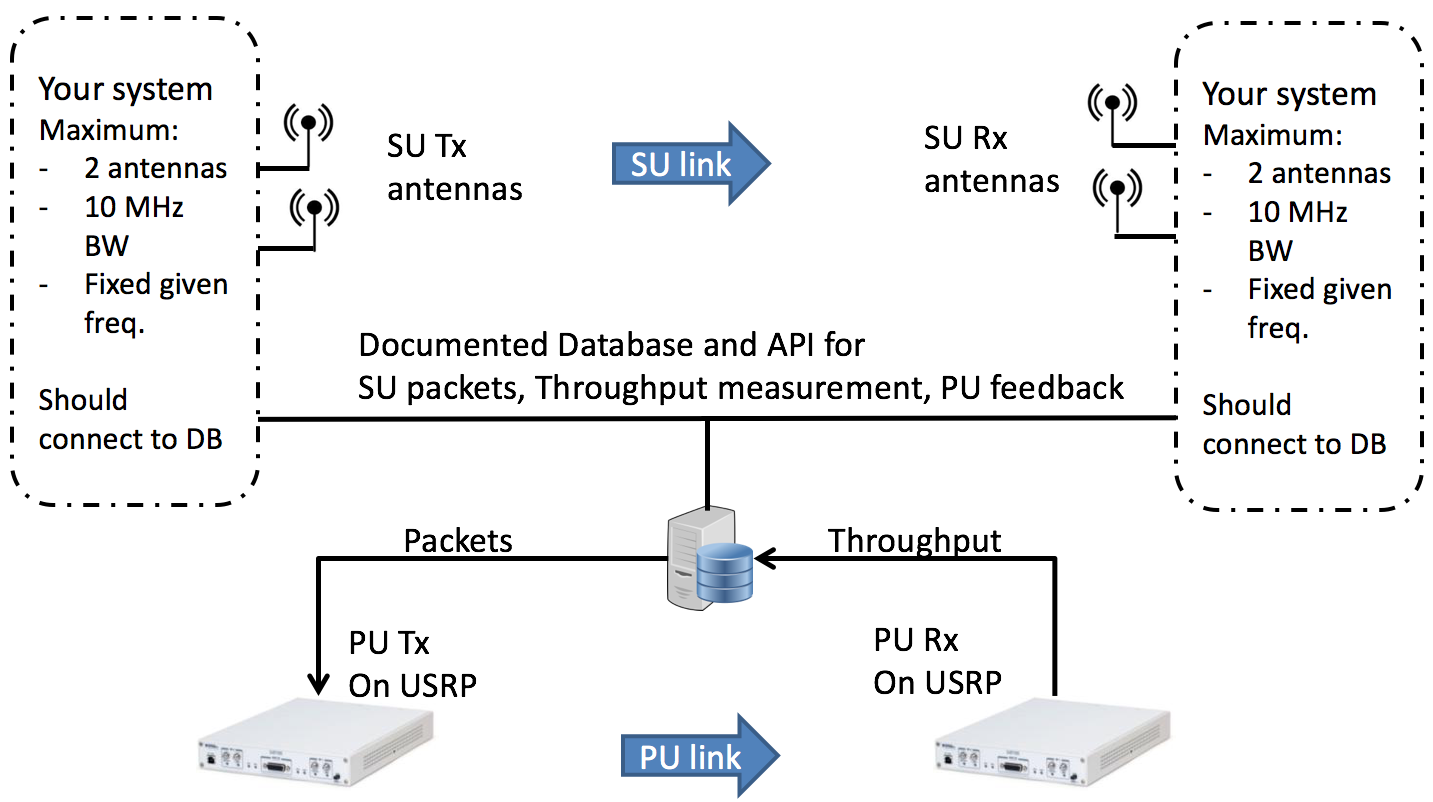
\includegraphics[width=0.8\textwidth]{figures/dyspan_set.png}
      \caption{The DySpan Spectrum Challenge Setup \cite{Dyspanchalle}}
      \label{fig:dyspan_setup}
\end{figure}

By using this configuration and keeping the hardware and overall physical considerations (such as \ac{BW}, number of antennas and central frequency),
the idea of the challenge was to achieve the maximum throughput between the proposed \ac{SU} systems, while interfering as little as possible with the existing \ac{PU}. The competition consisted of two phases: during phase one the situational awareness of the proposed \ac{CR} system is put under test, as it is needed to correctly identify the set of \ac{PU} transmission parameters:

\begin{itemize}
    \item Bandwidth and Carrier Frequency: Along the 10MHz of maximum \ac{BW} divided into four subchannels of 2.5MHz each, it needs to be detected if the \ac{PU} is using one, two or four channels for its transmission. Effectively, it is needed to determine which frequencies are being used (identify the frequency hopping pattern) and when are they being used.
    \item Packed length: The \ac{PU} transmitter sends packets in a bursty fashion to the corresponding receiver using packets of 64B payload.
    \item Inter-arrival time between packets: the time between a packet transmission might vary from a situation to another. These times could be deterministic for some scenarios, as well as stochastic for others following a Poisson distribution. Correctly identifying the interpacket time of the current situation, allows for effective opportunistic access to the spectrum.
\end{itemize}

With these characteristics, a set of 10 different scenarios is built, whose parameters are depicted in Table~\ref{table:scenarios}.

\begin{table}[h!]
    \centering
    \caption{Scenario description}
    \label{table:scenarios}
    \begin{tabular}{| >{\centering}m{5em}| m{12cm} |}
        \hline
        \textbf{Scenario} & \multicolumn{1}{|c|}{\textbf{Description}} \\
        \hline\hline
        0 & Single random channel, deterministic interpacket delay of 5ms \\\hline
        1 & Single random channel, deterministic interpacket delay of 10ms\\\hline
        2 & Two random channel hopping, deterministic interpacket delay of 5 ms\\\hline
        3 & Four random channel hopping, deterministic interpacket delay of 10 ms\\\hline
        4 & Two random channel hopping, deterministic interpacket delay of 5ms\\\hline
        5 & Four synchronous channels, deterministic interpacket delay of 5ms\\\hline
        6 & Four synchronous channels back-to-back, deterministic interpacket delay of 2ms\\\hline
        7 & Four asynchronous random channels, Poisson distributed interpacket delay with mean of 20ms\\\hline
        8 & Four asynchronous random channels, Poisson distributed interpacket delay with mean of 10ms\\\hline
        9 & Four asynchronous random channels, Poisson distributed interpacket delay with mean of 5ms\\
        \hline
    \end{tabular}
\end{table}

The second phase of the competition regards the benchmark of the performance of the proposed \ac{SU} implementation, where aspects such as innovation of the used waveform, \ac{ML} algorithms used, and opportunistic access to the spectrum were considered. The proposed solutions, including the one proposed by \ac{CEL}, can be found at \cite{Wunsch2017a}, \cite{Papadakis2017}, \cite{Paisana2017} and \cite{Lackpour2017}, where a high level of innovation and state-of-the-art research is compiled.

Being clear that \emph{awareness} has been a primordial characteristic of \ac{CR} since the conception of the concept until now, understanding that this is an area that invites to further research and considering the uprising research in the field of \ac{AI} algorithms, this work focuses on the learning aspect of \ac{CR}, using the setup from Fig.~\ref{fig:dyspan_setup} in order to effectively identify the scenarios described at Table~\ref{table:scenarios}. Previous research on this field covers aspects such as modulation recognition \cite{Oshea2016}\cite{Oshea2016d}, resource allocation \cite{Zappone2016}, autoencoding and optimization of MIMO systems \cite{Oshea2017}, dynamic spectrum management \cite{Haykin2005} and context awareness \cite{Paisana2017}\cite{Wunsch2017}.


The outline of this thesis is as follows: an introduction to \ac{AI}, focused on \ac{ML} and \ac{DL}, alongside the most used algorithms used in academic and industrial fields is presented in chapter~\ref{ch:ml_intro}. General techniques to avoid phenomena such as underfitting and overfitting of the \ac{ML} are, as well, portrayed. Chapter~\ref{ch:implementation} describes the details of the testbed setup, the measurement of the data and the implementation of the \ac{ML} models. The evaluation of the learning models is then presented in chapter~\ref{ch:evaluation} with metrics of performance. The models are put into a live implementation, where the performance of the algorithms is evaluated by classifying the scenarios of Table~\ref{table:scenarios} in real-time - This is presented in chapter~\ref{ch:live}. Lastly, the conclusions and future work are summarized in chapter~\ref{ch:conclusions}.
